\section{Data and Trigger}

The data used for this analysis was recorded in May 2010 at a centre of mass energy of 7 TeV. The average number of proton-proton collisions per bunch crossing during this period of data taking was estimated as less then 0.1. As a result the dataset is dominated by events involving a single proton-proton interaction; with only a small contribution of events with multiple proton-proton interactions. The data is separated into two subsets:  events recorded with the LHCb magnet field down or up. The dataset consists of 5.8 million and 12.2 million events respectively for down and up magnet configurations. The Monte Carlo simulated data are also divided into magnet up and magnet down configurations, both consisting of 35 million events. The simulated events are constrained to events with only one proton-proton interaction in order to emulate the data.

The track selection consists of long tracks (see section \ref{subsection: tracking, track reconstruction}) together with several kinematic requirements that select tracks from regions where the detector efficiency is high and background contributions are small. A momentum requirement of $p \ge 2$ GeV and $p_T \ge 0.2$ GeV removes low momentum tracks; pseudorapidity requirement of $2.0 \le \eta < 4.8$ selects tracks corresponding to particles that have transversed a greater number of tracking stations due to the geometry and positioning of the tracking stations, and a requirement on the proximity of the track to the mean interaction region (described in the section \ref{section: interaction region}). These selections require that the minimum distance between the track and mean interaction region (Distance Of Closest Approach, DOCA) is 2 mm and that the the track is within 3 standard deviations of the mean z position of the mean interaction region (figure \ref{fig: track selection criteria}). This requirement ensures that particles that are produced far away from the interaction region (i.e. unlikely to be prompt particles) do not pass the selection. The track selections are shown in figure \ref{fig: track selection criteria}

The trigger requirements for the data are minimal, requiring at least one selected track is reconstructed in events where the beams are registered as crossing.

\begin{figure}[h]
	\begin{subfigure}[h]{0.49\textwidth}
		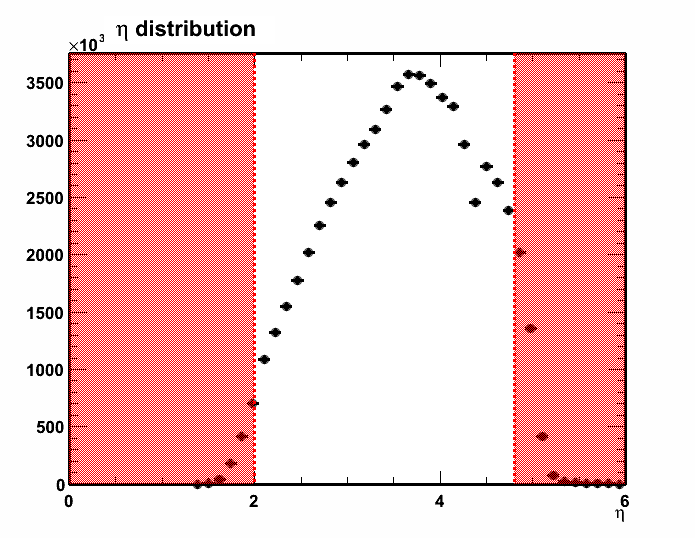
\includegraphics[width=\textwidth]{./Chapters/multiplicity/images/track_selection_eta.png}
		\caption{$\eta$}
		\label{fig: track selection criteria eta}
	\end{subfigure}
	\begin{subfigure}[h]{0.49\textwidth}
		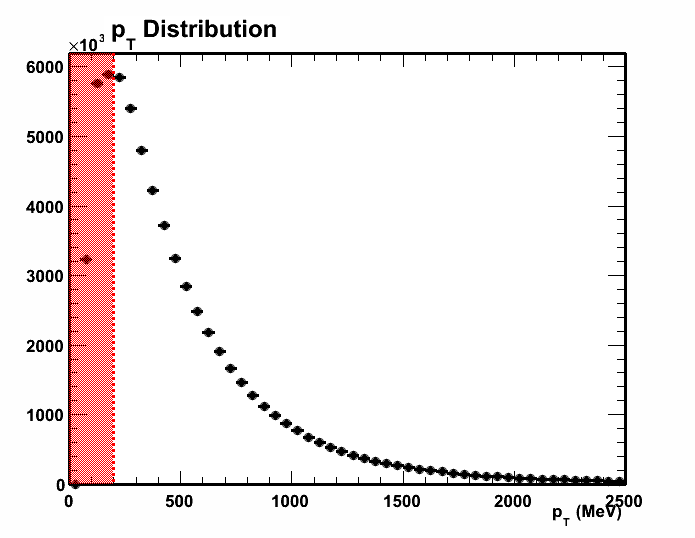
\includegraphics[width=\textwidth]{./Chapters/multiplicity/images/track_selection_pt.png}
		\caption{$p_T$}
		\label{fig: track selection criteria pt}
	\end{subfigure}
	\begin{subfigure}[h]{0.49\textwidth}
		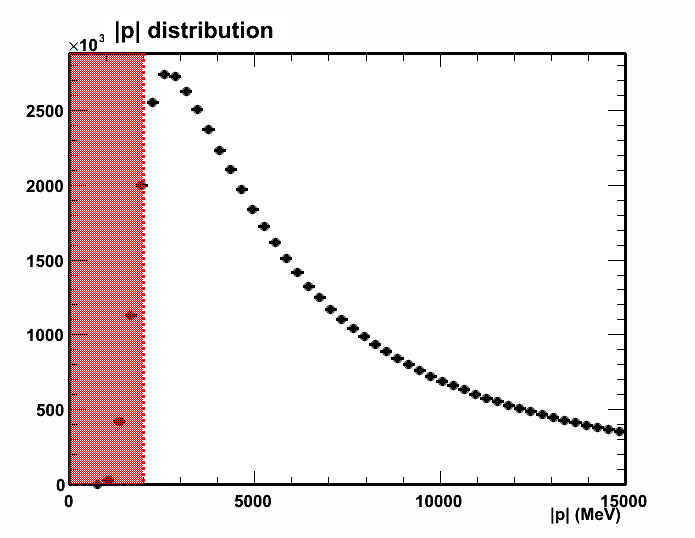
\includegraphics[width=\textwidth]{./Chapters/multiplicity/images/track_selection_p.png}
		\caption{$|p|$}
		\label{fig: track selection criteria p}
	\end{subfigure}
	\begin{subfigure}[h]{0.49\textwidth}
		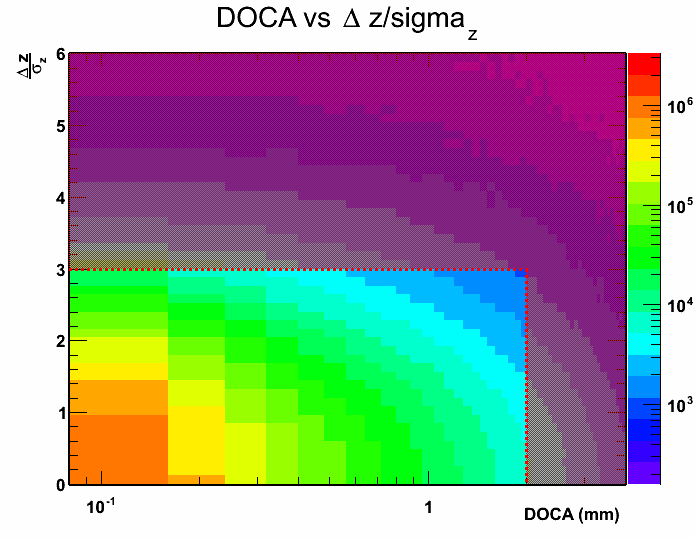
\includegraphics[width=\textwidth]{./Chapters/multiplicity/images/track_selection_ir.png}
		\caption{Interaction region}
		\label{fig: track selection criteria ir}
	\end{subfigure}
	\caption{Track selection criteria}
	\label{fig: track selection criteria}
\end{figure}